%%
%% This is file 'sample-degree-report.tex' was based on the ACM's`sample-manuscript.tex'.
%% Note that this was taken from the Overleaf project: https://www.overleaf.com/gallery/tagged/acm-official#.WOuOk2e1taQ
%% It has been adapted to use the TIMTM template (adapted from CHI Proceedings Template) for
%% the Interactive Media Technology (TIMTM) and Media Management (TMMTM) programmes at KTH Royal Institute of Technology.
%% 
%% 2021-11-09 Gerald Q. Maguire Jr. adapted template to KTH's TITM and TMMTM requirements, including:
%% removing the ACM copyright and other notices in the generate documents - as these are not applicable
%% and rewriting some of the contents of the sample document.§
%%
%% IMPORTANT NOTICE:
%% 
%% For the copyright see the file: acmart-primary/acmart.dtx - from the github
%%
%% The first command in your LaTeX source must be the \documentclass command.

%%%% Generic manuscript mode, required for submission
%%%% and peer review
%\documentclass[manuscript,screen,review]{timtm}
\documentclass[screen, sigcconf]{timtm}
%% Fonts used in the template cannot be substituted; margin 
%% adjustments are not allowed.
%%
%% \BibTeX command to typeset BibTeX logo in the docs
\makeatletter%
\@ifclassloaded{acmart}%
  {\AtBeginDocument{%
  \providecommand\BibTeX{{%
   \normalfont B\kern-0.5em{\scshape i\kern-0.25em b}\kern-0.8em\TeX}}}}%
  {\AtBeginDocument{%
  \providecommand\BibTeX{{%
   \rm B\kern-.05em{\sc i\kern-.025em b}\kern-.08em\TeX}}}}%
\makeatother%



%% Note that it you do happen to repurpose this file for a submission to SIGCHI, you might add the line below - as you need to retain the copyright, since KTH must be able to distribute copies upon request.
\setcopyright{rightsretained}

\copyrightyear{2021}

%% For an actual ACM submission
%% Rights management information.  This information is sent to you
%% when you complete the rights form.  These commands have SAMPLE
%% values in them; it is your responsibility as an author to replace
%% the commands and values with those provided to you when you
%% complete the rights form.
%\setcopyright{acmcopyright}
%\copyrightyear{2018}
%\acmYear{2018}
%\acmDOI{10.1145/1122445.1122456}

%% These commands are for a PROCEEDINGS abstract or paper.
%\acmConference[Woodstock '18]{Woodstock '18: ACM Symposium on Neural  Gaze Detection}{June 03--05, 2018}{Woodstock, NY}
%\acmBooktitle{Woodstock '18: ACM Symposium on Neural Gaze Detection,  June 03--05, 2018, Woodstock, NY}
%\acmPrice{15.00}
%\acmISBN{978-1-4503-XXXX-X/18/06}


%%
%% Submission ID.
%% Use this when submitting an article to a sponsored event. You'll
%% receive a unique submission ID from the organizers
%% of the event, and this ID should be used as the parameter to this command.
%%\acmSubmissionID{123-A56-BU3}

%%
%% Use numbered citations and references. 
%%

%% If the acmart document class is being used, define away some commands and environment
%% If not, then enable ISBNs to be shown in references
\makeatletter%
\@ifclassloaded{acmart}%
{%
\newcommand{\alttitle}[1]{}
\newcommand{\altsubtitle}[1]{}
\newenvironment{swedishabstract}{}{}
\newcommand{\SwedishKeywords}[1]{}
}{%
% Define these so that the bibliography will include ISBNs
\newcommand{\showISBNx}{}
\newcommand{\showISBNxiii}{}
}%
\makeatother%


%% end of the preamble, start of the body of the document source.
\begin{document}

%%
%% The "title" command has an optional parameter,
%% allowing the author to define a "short title" to be used in page headers.
\title{A Visual Programming Language In Virtual Reality}
\subtitle{An Evaluation using Cognitive Dimensions and Health Metrics}

% give the alternative title - i.e., if the thesis is in English, then give a Swedish title
\alttitle{Detta är den svenska översättningen av titeln}
\altsubtitle{Detta är den svenska översättningen av undertiteln}

%%
%% The "author" command and its associated commands are used to define
%% the authors and their affiliations.
%% Of note is the shared affiliation of the first two authors, and the
%% "authornote" and "authornotemark" commands
%% used to denote shared contribution to the research.
\author{Adam Jonsson} 
%\authornote{Both authors contributed equally to this research.}
\email{adajon@kth.se}
% Apply the same authornote for the second author
%\orcid{1234-5678-901X}
\affiliation{%
  \institution{KTH Royal Institute of Technology, School of Electrical Engineering and Computer Science}
  %\streetaddress{Streat address}
  \city{Stockholm}
  \country{Sweden}
  \postcode{SE 100 44}
}

%%
%% The abstract is a short summary of the work to be presented in the
%% article.
\begin{abstract}
  This sample report describes the formatting
  requirements for a Interactive Media Technology (TIMTM) and Media Management (TMMTM) programmes at KTH Royal Institute of Technology. It is based upon the ACM conference proceedings format, and offers
  recommendations on writing for the worldwide SIGCHI
  readership. Please review this document, as some format details have changed
  relative to previous years. Abstracts should be about 150 words.
  
  All theses at KTH are \textbf{required} to have an abstract in both \textit{English} and \textit{Swedish}.
\end{abstract}

\begin{swedishabstract}
Alla avhandlingar vid KTH \textbf{måste ha} ett abstrakt på både \textit{engelska} och \textit{svenska}.

Om du skriver din avhandling på svenska ska detta göras först (och placera det som det första abstraktet) - och du bör revidera det vid behov.
\end{swedishabstract}

%%
%% The code below is generated by the tool at http://dl.acm.org/ccs.cfm.
%% Please copy and paste the code instead of the example below.
%%
\begin{CCSXML}
<ccs2012>
 <concept>
  <concept_id>10010520.10010553.10010562</concept_id>
  <concept_desc>Computer systems organization~Embedded systems</concept_desc>
  <concept_significance>500</concept_significance>
 </concept>
 <concept>
  <concept_id>10010520.10010575.10010755</concept_id>
  <concept_desc>Computer systems organization~Redundancy</concept_desc>
  <concept_significance>300</concept_significance>
 </concept>
 <concept>
  <concept_id>10010520.10010553.10010554</concept_id>
  <concept_desc>Computer systems organization~Robotics</concept_desc>
  <concept_significance>100</concept_significance>
 </concept>
 <concept>
  <concept_id>10003033.10003083.10003095</concept_id>
  <concept_desc>Networks~Network reliability</concept_desc>
  <concept_significance>100</concept_significance>
 </concept>
</ccs2012>
\end{CCSXML}

\ccsdesc[500]{Computer systems organization~Embedded systems}
\ccsdesc[300]{Computer systems organization~Redundancy}
\ccsdesc{Computer systems organization~Robotics}
\ccsdesc[100]{Networks~Network reliability}

%%
%% Keywords. The author(s) should pick words that accurately describe
%% the work being presented. Separate the keywords with commas.
\keywords{datasets, neural networks, gaze detection, text tagging}
% The following adds the Swedsih version of your keywords
\SwedishKeywords{datauppsättningar, neurala nätverk, blickdetektering, texttaggning}

%% In a SIGCHI submission you can include a teaserfigure:
%% A "teaser" image appears between the author and affiliation
%% information and the body of the document, and typically spans the
%% page.
%\begin{teaserfigure}
%  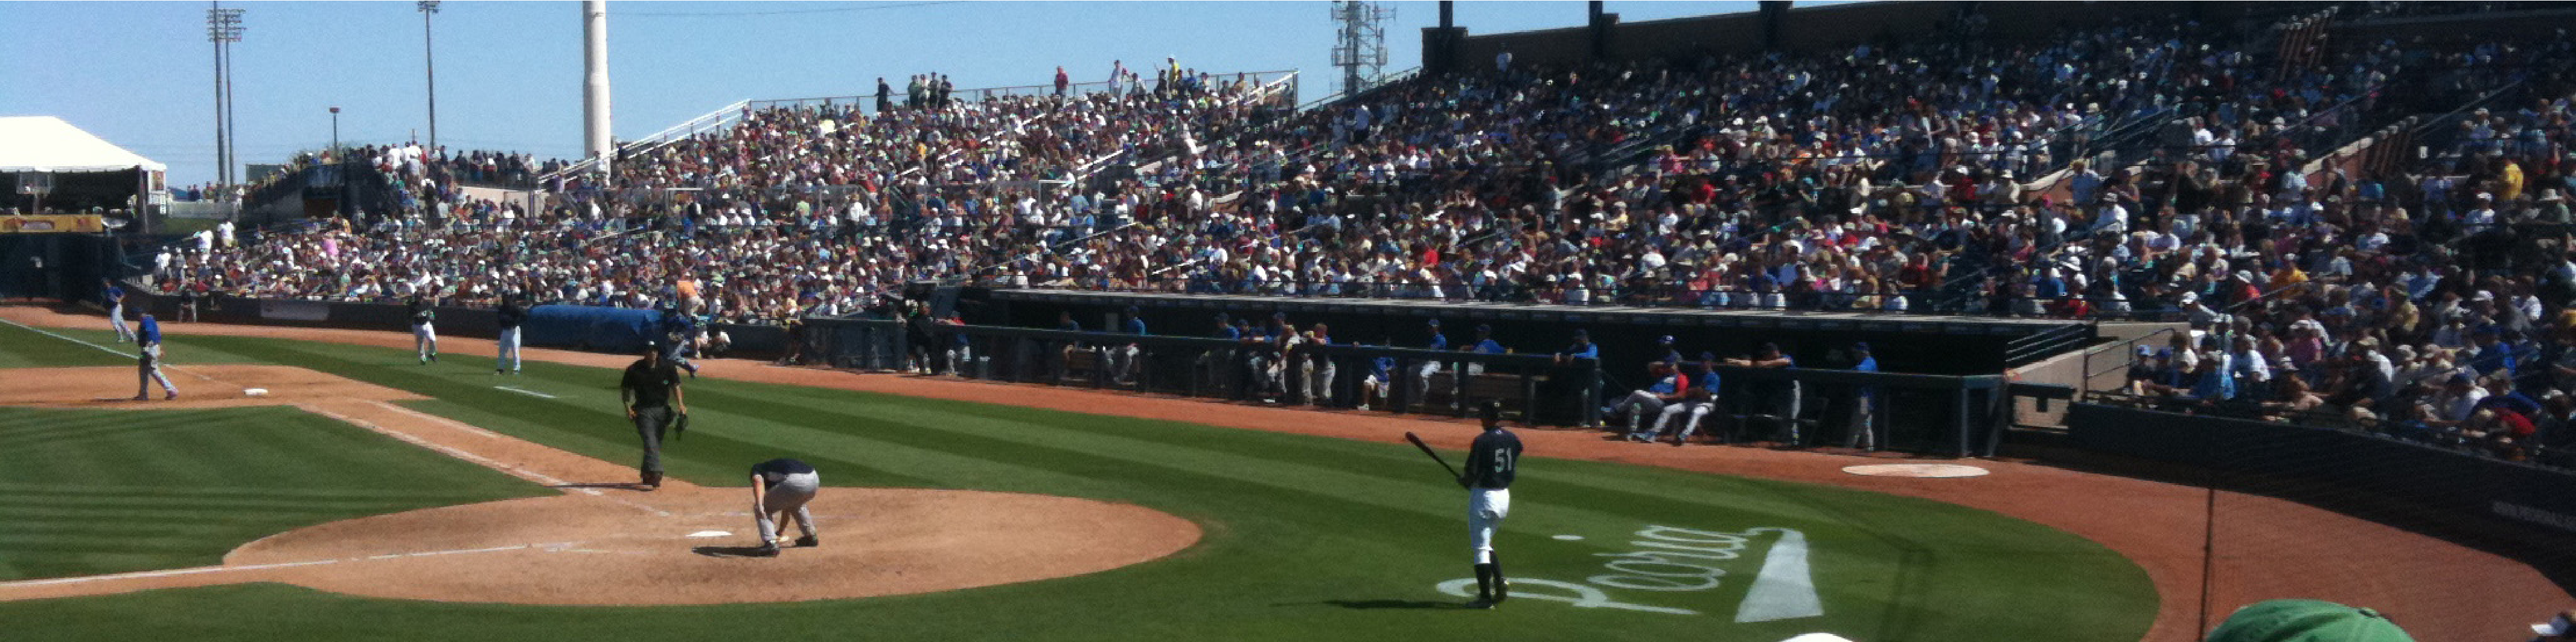
\includegraphics[width=\textwidth]{sampleteaser}
%  \caption{Seattle Mariners at Spring Training, 2010.}
%  \Description{Enjoying the baseball game from the third-base
%  seats. Ichiro Suzuki preparing to bat.}
%  \label{fig:teaser}
%\end{teaserfigure}
%

%%
%% This command processes the author and affiliation and title
%% information and builds the first part of the formatted document.
\maketitle

\section{Introduction}

Professions that are primarily conducted sedentary have increased due to the growth of office-related occupation \cite{parry_contribution_2013}. One such profession is software engineering. A concern with this direction is that sedentary behavior has been found to have a negative effect on a person's health, such as obesity \cite{lakdawalla_labor_2007}, depression \cite{zhai_sedentary_2015}, and a higher risk of cardiovascular events \cite{straker_sedentary_2016}. Therefore, it is of interest to reduce sedentary, making the work environment healthier.

There exist previous studies exploring ways to prevent sedentary behavior during work, such as making the employers more aware of their activity with the help of notification from a mobile application \cite{cole_they_2015}, introducing standing desks \cite{pronk_reducing_2012}, and walking while having meetings \cite{bort-roig_uptake_2014}. One of these studies found that to make the change be of effect, the intervention can not hurt the productivity and needs to be customized for the work context \cite{bort-roig_uptake_2014}.

% Similarly, this degree project aims to explore the potential to reduce the sedentary behavior for software engineers. But instead of adding intervention to the work environment, this study explores the potential of conducting software engineering in virtual reality that requires movement, reducing the sedentary behavior form the work itself.

Another potential means of reducing sedentary behavior is using virtual reality (VR) during work. This is because a VR device that uses six degrees of freedom has its benefit in that it requires more movement than sitting in front of a computer. A typical VR application might need users to walk, look around, and move their arms to grab or push interactable. Of course, the design of a VR application heavily affects the frequency at which these movements occur. Compare this to a mouse and keyboard setup, where the user only needs to do small movements with their fingers and wrist to interact with a GUI. One meta-analysis on physical training in VR concluded that the technology has potential \cite{ng_effectiveness_2019}

While VR can be beneficial in increasing movement, one potential issue with conducting software engineering inside VR is the performance. Software engineering as an occupation often requires programming, which is typically done with the help of a keyboard. One study has found that many typing technics with VR controllers are significantly slower compared to using a qwerty keyboard \cite{speicher_selection-based_2018}. Therefore, generating code by typing inside VR might prevent sedentary behavior but potentially reduce productivity.

\begin{figure}[h]
  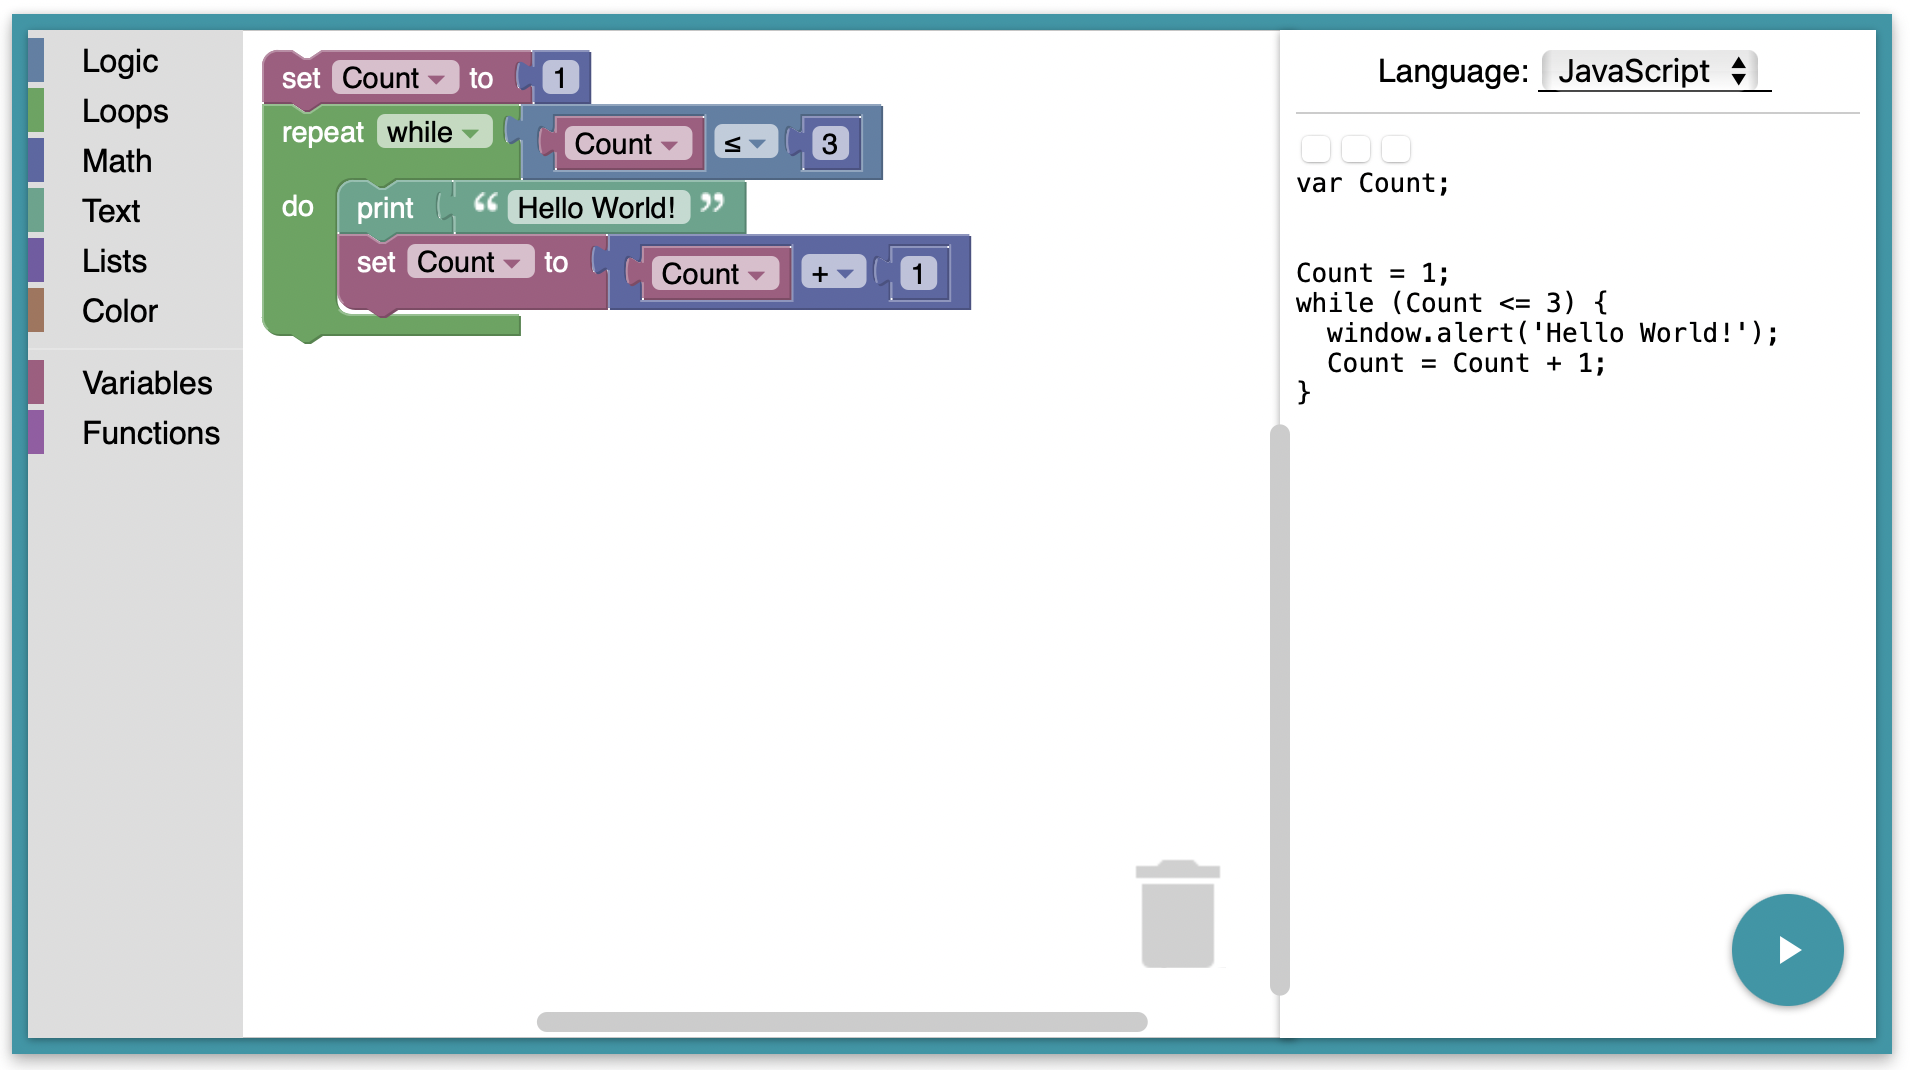
\includegraphics[width=\linewidth]{figures/blockly.png}
  \caption{Example of code inside Blockly}
  \label{fig:blockly}
\end{figure}

% Change this & fix references
One approach that does not primarily requires text entry input is using a visual programming language (VPL). That is, one needs to move elements around in a program in order to create the desired outcome. There are mainly two types of VPL. One is a block-based approach, similar to putting lego together, which is forcing a specific layout of the code blocks \cite{mason_block-based_2017}. The other is a flow-based approach which is more like putting cables together and is instead more free regarding placement of the code \cite{mason_block-based_2017}. Blockly is a popular block-based open source VPL published by Google and has been shown to be easy to understand and get started with \cite{seraj_scratch_2019}, see figure \ref{fig:blockly}. Blockly is built using code blocks, each block representing a type of code. The green one seen in figure \ref{fig:blockly} is, for example, a while loop, while the light blue is a logic comparator.

VPLs have previously been implemented in VR. For example, FlowMatic \cite{zhang_flowmatic_2020} is a flow-based environment for creating VR applications, while Cubely \cite{vincur_cubely_2017} makes use of blocks for teaching programming. HackVR \cite{kao_hackvr_2020} combines the flow-based approach with the object-oriented paradigm. However, none of these studies focused on the health aspect or compared the performance of doing a VPL in front of a computer.

However, a potential challenge in making a VPL inside VR that is both performant and contributes to movement is that those two factors might work against each other. That is, the more movement the application requires, the less performant it will be, and vice versa. For example, having interactable objects further apart from each other will make the user need to move more. However, it will hurt productivity as the user needs to move forth and back, as compared to them having them close together. A VPL inside VR might have such issues depending on its design. However, there are types of interactions in a VPL inside VR other than walking, such as connecting code blocks, restructuring current, and navigating around the code space. These other interactions may have movement/performance relationships that differ from moving between points A and B. Not knowing these relationships or performance differences can make designing a VPL in VR challenging. Therefore, identifying these relationships and comparing the performance to doing VPL on a computer can help accelerate the development of a performant VPL inside VR. Which in turn can be used to reduce sedentary behavior for software engineers.

To conclude, in this degree project, the potential of reducing sedentary behavior for software engineering using virtual reality will be explored. More specifically, performance differences in relation to movement between coding in a VPL inside virtual reality and a computer will be measured. This degree project aims to contribute to future researchers and designers in creating an efficient visual programing language inside virtual reality that can reduce sedentary behavior while also being performant.

\section{Background}

\subsection{Virtual Reality}

\subsubsection{Health}
A potential means of reducing sedentary behavior is using virtual reality (VR) during work. This is because a VR device that uses six degrees of freedom has its benefit in that it requires more movement than being sedentary in front of a computer. A typical VR application might need users to walk, look around, and move their arms to grab or push interactable. Of course, the design of a VR application heavily affects the frequency at which these movements occur. Compare this to a mouse and keyboard setup, where the user only needs to do small movements with their fingers and wrist to interact with a GUI. One meta-analysis on physical training in VR concluded that the technology has potential \cite{ng_effectiveness_2019}

\subsubsection{Text-entry Input}
One issue with VR using hand controllers is the text-input performance. The reason is that current two hand controllers have a limited number of buttons compared to a QWERTY keyboard. As a result, text-input in VR often take use of hand movement, also called select based typing. Marco Speicher et al. explored multiple variation of select base typing and compared the performance to traditional keyboard input \cite{speicher_selection-based_2018}. The multiple select based typing includes: 1) Head pointing, using the head to point at the letter that the user wants to select. 2) Controller pointing, using both controllers to point to letters that the user wants to select. 3) Controller tapping, physically tapping the letters with the controllers. 4) Freehand, using hand tracking were the user is typing on a virtual keyboard. 5) Discrete and continuous cursor, the user uses the buttons on the controller to move a cursor on the keyboard. Their findings was that controller pointing was the most performant in terms of WPM, as well as having the lowest error rate. It was also the most liked by the participants and had the least amount of frustration. However, while controller pointing was the most performant with an average words per minute (WPN) around 15, it falls short compared to keyboard typing with a WPN of 50. It is worth to mention that the study had a fixed distance and size between the user and the virtual keyboard for all different select based typing. Different distances and sizes could therefore potentially give different outcome.

\subsubsection{Motion Sickness}
Motion sickness is the phenomenon were the user feel sick after using a VR headset a while. The amount and frequency of motion sickness varies depending on the design of the VR application and the individual resistance to motion sickness. In VR, the cause of motion sickness is mostly due to sensory conflict where movement occur in the virtual world but not in the real physically one \cite{golding_motion_2006}. An example where this can occur is when there is continuous movement by using a joystick to traverse the virtual world without needing to physically move. With six degree of freedom headset, the user can physically move to move in the virtual world, preventing sensory conflict and thus motion sickness. However, limited physically space is one reason why physically movement is not always used to move in the virtual world.

\subsubsection{Accommodation-Vergence Mismatch}
Retinal cues of disparity and blur makes the eyes change accommodation and vergence in order to create one clear image \cite{reichelt_depth_2010}. Accommodation is when the eyes change its focus to create a clear image of what is looked at. If the accommodation fails, the object that is looked at is going to be perceived blurry. Vergence is when the eyes converge or diverge from each other to create a singel image. If vergence fails, visual disparity is perceived, making the object that is looked at appear twice. Accommodation and vergence have been found to be influencing each other, meaning that when accommodation changes, vergence also changes as a reflex, and vice versa \cite{suryakumar_vergence_2007}. Because of this, it is difficult only change accommodation or vergence without changing the other.

In the context of virtual reality headsets, there is a phenomenon called accommodation-vergence mismatch, also called accommodation-vergence conflict \cite{kramida_resolving_2016}. This causes objects to close to the viewer to be blurry or to appear twice. The reson for this is that most VR headsets uses fixed lenses, resulting in a fixed focal length of the viewed content. This means that the user do not need to change their accommodation when using VR. However, the viewer need to alter their vergence due to VR using stereoscopic displays that creates the illusion of 3D. Requiring the viewier to have a fixed accommodation while changing their vergence can cause a accommodation-vergence mismatch, see figure \ref{fig:accommodation_vergence_conflict}. For viewing objects far away, the mismatch is at a level that it is not noticeable for the viewer. However, when object are too close to the headset, the mismatch is at a level that the vision either becomes blurry or have disparity \cite{hoffman_vergenceaccommodation_2008}. This can lead to eye-strain, eye-tiredness and headache \cite{shibata_zone_2011}. For this reason, the viewable content in VR should be placed a a distance such that it minimize accommodation-vergence mismatch.

\begin{figure}[h]
  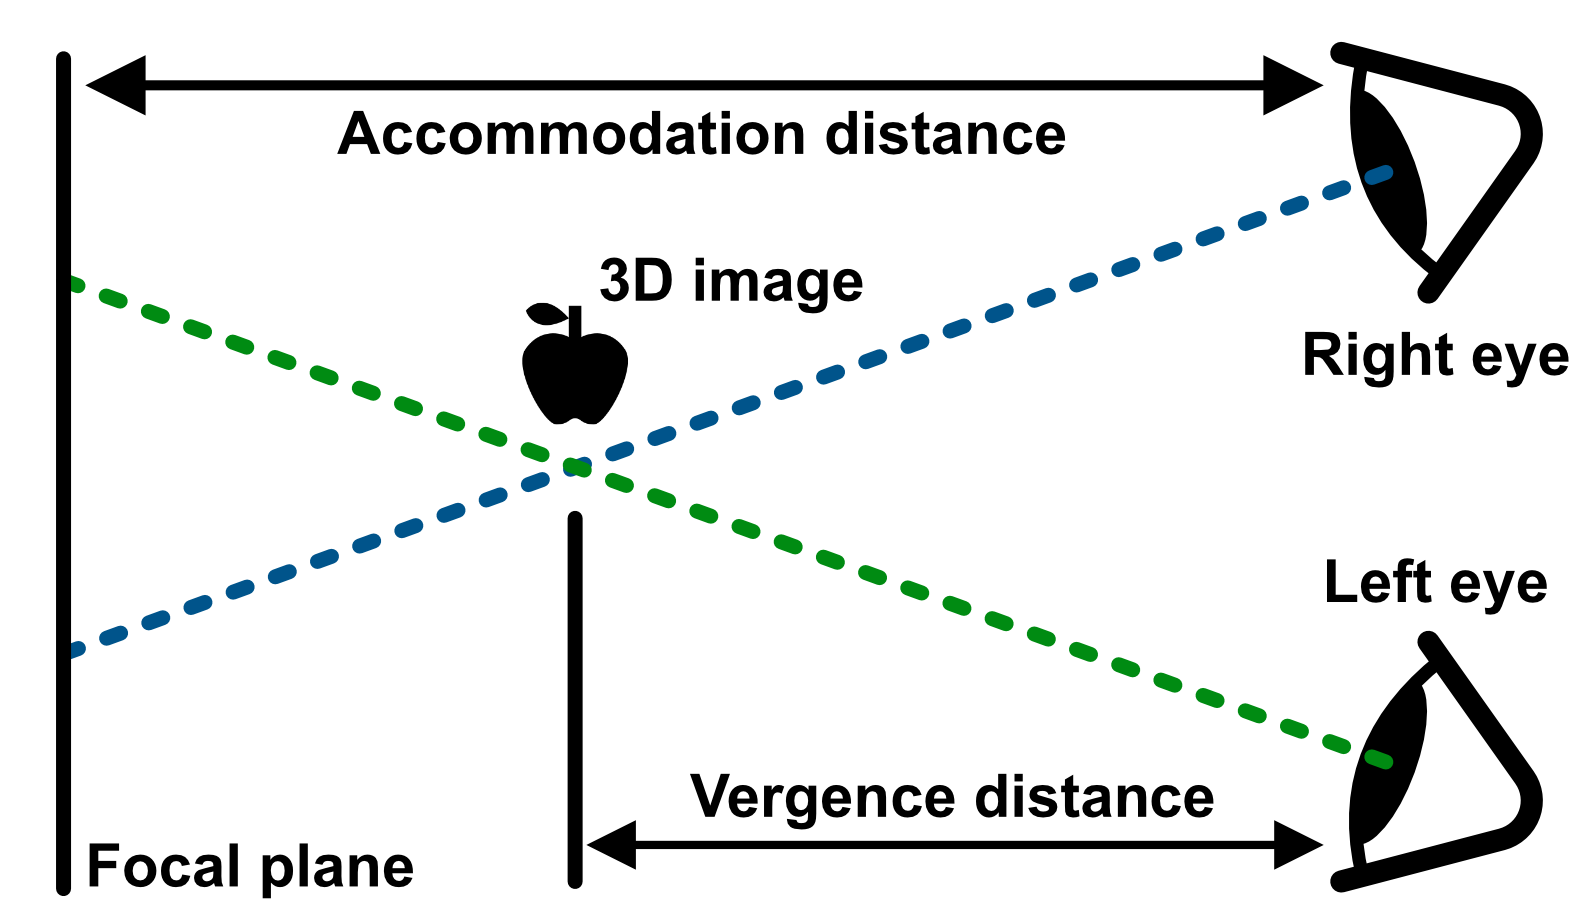
\includegraphics[width=\linewidth]{figures/AccommodationVergenceConflict.png}
  \caption{Example of accommodation and vergence having difference distances, also called accommodation-vergence mismatch}
  \label{fig:accommodation_vergence_conflict}
\end{figure}

On study have mapped the viewing distance such that accommodation-vergence mismatch is at a comfortable level \cite{shibata_zone_2011}. They found that discomfort is more promoment when the vergence distance is shorter than the accommodation distance, rather than longer. Looking at figure \ref{fig:comfort_viewing_diagram}, a Oculus Quest 2 headset that has a focal length of 1.3 meter, has a comfortable viewing range about 0.6 meter and more. This is in accordance with the minimum 0.5 meter distance Meta recommends \cite{noauthor_vision_nodate}

\begin{figure}[h]
  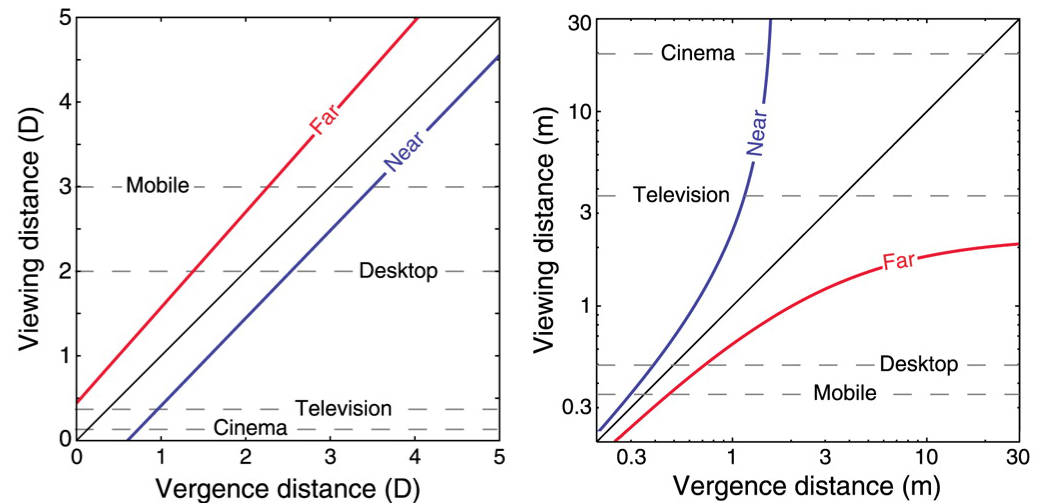
\includegraphics[width=\linewidth]{figures/ComfortViewingDiagram.png}
  \caption{Comfortable viewing distances in terms of accommodation-vergence mismatch}
  \label{fig:comfort_viewing_diagram}
\end{figure}

\subsection{Cognitive Dimensions of Notations}
The framework Cognitive Dimensions of Notations, also called CDs, was introduced by XXX with the main goal to provide a vocabulary for design choices in notational systems, as well as an analytic method for a systems usability. The CDs framework have been used in multiple studies \cite{hadhrawi_systematic_nodate}, one of which is a VPL based on Blockly by XXX and XXX \cite{holwerda_usability_2018}. This particularly study based their VPL on Blockly, same as this study. For this reason, the findings is used as a base for some of the design choice of the VPL in VR in this study.

The reason the CDs framework is used to evaulate a VPL in VR is that it is not focusing on the details and perfomance of the application. More detailed evaulation, such as performance and error rate is not the primary focus on this early research area and prototype. Instead, the focus is to evaluate the different dimensions of using a VPL inside VR, both in terms of usability and movement. That is, there might be interactions that works well in VR and other that do not, some that contribute to movement but lack in a given CDs. Identifying these advandates and disadvandates with a well research framework can help future designers and researchers use the findings. 

Moreover, the focus is on dimensions that is affected by the three-dimensional envoriement which virtual reality enables. These include:

The dimensions of the CDs framework include:

\subsubsection{Visibility: Ability to View Components Easily}

\subsubsection{Viscosity: Resistance to Change}

\subsubsection{Premature Commitment: Constraints on the Order of Doing Things}

\subsubsection{Hidden Dependencies: Important Links between Entities Are Not Visible}

\subsubsection{Role-Expressiveness: The Purpose of an Entity Is Readily Inferred}

\subsubsection{Error-Proneness: The Notation Invites Mistakes and the System Gives Little Protection}

\subsubsection{Abstraction: Types and Availability of Abstraction Mechanisms}

\subsubsection{Secondary Notation: Extra Information in Means Other Than Formal Syntax}

\subsubsection{Closeness of Mapping: Closeness of Representation to Domain}

\subsubsection{Consistency: Similar Semantics Are Expressed in Similar Syntactic Forms}

\subsubsection{Diffuseness: Verbosity of Language}

\subsubsection{Hard Mental Operations: High Demand on Cognitive Resources}

\subsubsection{Provisionality: Degree of Commitment to Actions or Marks}

\subsubsection{Progressive Evaluation: Work-to-Date Can Be Checked at Any Time.}



* (Source) Providing a vocabulary
  * (Source) There are other techniques for analyzing the usability of computer systems, but these often focus on the finest details of interaction 
* Are there coginitve dimensions system within systems?
* (Source) The frameworks provides a way to identify tradeofs for different designs. If you increase visiblity to may cuse 
* TODO: Say that we are not focusing on the keyboard aspects, etc.
* (Source) The different dimensions are not orthogonal, that is, a design change in one dimension can effect another dimension both positive and negatively.



\section{Design}

\subsection{Blocks}
Talk about the final design for the blocks

\subsection{Menus}
Talk about the final design for the menus

\section{Method}
The research methodology is design-based research. TODO: The reason being that the area of research is fairly new, etc.

There are two primary areas that are going to be evaluated. The first one is the health aspect wi

\subsection{Cognitive Dimensions Questioner}
The authors of Cognitive Dimensions, Thomas R.G Green and Alan F. Blackwell, created a questioner that could be used to evaluate the usability of environment, tools, and programming languages \cite{blackwell_cognitive_2000}. The proposed questions in the questioner is design such that it can be applied to any system. (Say that it works before specifying the down sides and challanges of using it) However, the questioners general results in it being harder for the user to understand what part of the system relates the a given question. This was both confirmed in the pilot study when evaluating the CDs questioner \cite{blackwell_cognitive_2000} and another study evaluating a VPL based on Blockly\cite{holwerda_usability_2018}. Still, the gathered data for both studies were useable. Moreover, the CD questioner is also designed for users that are experienced with the system being evaluated, which could potentially make the questioner hard for the participants in this study that are completely new to the VR-application. There is therefore of interest of modifying the questions of the  original questioner such that it becomes easier to understand and link the question to the VR application.

There are several issues using the questioner directly in this study. 

The 

\section{Template Overview}

This document will \emph{not} explain all the major features of the \verb|acmart| document
class, but will focus on the features of the \verb|timtm| document
class. The \verb|timtm| document
class is purposely similar to the \verb|acmart| document
class, thus facilitating your submitting your report to an ACM conference\footnote{Simply change the document class from timtm to acmart. This sample document conditionally redefines some commands and an environment - so that the features added for a degree project are not included in the resulting document.}. For further information about the details of the \verb|acmart| document
class, see the {\itshape \LaTeX\ User's Guide} --- 
available from \url{https://www.acm.org/publications/proceedings-template}.

The primary parameter given to the document class is
the {\itshape template style} which corresponds to the kind of publication. This parameter is enclosed in square
brackets and is a part of the {\verb|documentclass|} command:
\begin{verbatim}
  \documentclass[STYLE]{timtm}
\end{verbatim}

The styles relevant for a degree project report include:
\begin{itemize}
\item {\verb|sigcconf|}: The majority of ACM's conference proceedings use the {\verb|sigcconf|} template style, as will a degree project report for the Interactive Media Technology (TIMTM) and Media Management (TMMTM) programmes.
\item {\verb|screen|}: Produces colored hyperlinks.
\item {\verb|review|}: Includes line numbers.
\item {\verb|manuscript|}: Generally used in conjunction with \verb|review| to make it easy for a copy editor to work with your document.
\end{itemize}

\section{Modifications}

Modifying the template --- including but not limited to: adjusting
margins, typeface sizes, line spacing, paragraph and list definitions,
and the use of the \verb|\vspace| command to manually adjust the
vertical spacing between elements of your work --- is not allowed for actual ACM submissions\footnote{In the case of ACM submissions, your document will be returned to you for revision if modifications are discovered.} and are strongly discouraged for a degree project report --- let the template do lots of the work for you.

\section{Typefaces}

Degree project reports should use a Times Roman like font family, here we have used TeX Gyre. This is in contrast to the ``\verb|acmart|'' document class that requires the use of the ``Libertine'' typeface family.

\section{Title Information}

The title of your work should use capital letters appropriately -
\url{https://capitalizemytitle.com/} has useful rules for
capitalization. Use the {\verb|title|} command to define the title of
your work. If your work has a subtitle, define it with the
{\verb|subtitle|} command.  Do not insert line breaks in your title.

If your title is lengthy, you must define a short version to be used
in the page headers, to prevent overlapping text. The \verb|title|
command has a ``short title'' parameter:
\begin{verbatim}
  \title[short title]{full title}
\end{verbatim}

There are \verb|alttitle| and \verb|altsubtitle| commands so that you can easily specify a Swedish title and optionally a Swedish subtitle for your report. Note that both the thesis title and the Swedish thesis title will subsequently be entered as meta data in DiVA and in LADOK.

\section{Authors and Affiliations}

Each author must be defined separately for accurate metadata
identification. Multiple authors may share one affiliation. Authors'
names should not be abbreviated; use full first names wherever
possible. Include authors' e-mail addresses whenever possible. Note that grouping authors' names or e-mail addresses or e-mail
addresses is unacceptable.

The \verb|authornote| and \verb|authornotemark| commands allow a note
to apply to multiple authors --- for example, if the first two authors
of an article contributed equally to the work. The ``\verb|acmart|'' document class'  documentation, available at
\url{https://www.acm.org/publications/proceedings-template}, has a
complete explanation of these commands and tips for their effective
use.

\section{CCS Concepts and User-Defined Keywords}

Two elements of the ``acmart'' document class provide powerful
taxonomic tools for you to help readers find your work in an online
search.

The ACM Computing Classification System  (CCS) ---
\url{https://www.acm.org/publications/class-2012} --- is a set of
classifiers and concepts that describe the computing
discipline. Authors can select entries from this classification
system, via \url{https://dl.acm.org/ccs/ccs.cfm}, and generate the
commands to be included in the \LaTeX\ source.

User-defined keywords are a comma-separated list of words and phrases
of the authors' choosing, providing a more flexible way of describing
the research being presented.

For ACM submissions, CCS concepts and user-defined keywords are required for for all
articles over two pages in length, and are optional for one- and
two-page articles (or abstracts). For degree projects is is very desirable that you provide a suitable set of keywords to help potential readers find your thesis in DiVA.

There is a \verb|SwedishKeywords| command to make it easiy to add keyowrds in Swedish for your report. These can help make your report visible if someone searches for one or more of these Swedish keywords. You should order them in the same order that you entered the English keywords.

\section{Sectioning Commands}

Your work should use standard \LaTeX\ sectioning commands:
\verb|section|, \verb|subsection|, \verb|subsubsection|, and
\verb|paragraph|. They should be numbered; do not remove the numbering
from the commands.

Simulating a sectioning command by setting the first word or words of
a paragraph in boldface or italicized text is {\bfseries not allowed.}

\section{Tables}

The document class includes the ``\verb|booktabs|''
package --- \url{https://ctan.org/pkg/booktabs} --- for preparing
high-quality tables.

Table captions are placed {\itshape above} the table.

Because tables cannot be split across pages, the best placement for
them is typically the top of the page nearest their initial cite.  To
ensure this proper ``floating'' placement of tables, use the
environment \textbf{table} to enclose the table's contents and the
table caption.  The contents of the table itself must go in the
\textbf{tabular} environment, to be aligned properly in rows and
columns, with the desired horizontal and vertical rules.  Again,
detailed instructions on \textbf{tabular} material are found in the
\textit{\LaTeX\ User's Guide}.

Immediately following this sentence is the point at which
Table~\ref{tab:freq} is included in the input file; compare the
placement of the table here with the table in the printed output of
this document.

\begin{table}
  \caption{Frequency of Special Characters}
  \label{tab:freq}
  \begin{tabular}{ccl}
    \toprule
    Non-English or Math&Frequency&Comments\\
    \midrule
    \O & 1 in 1,000& For Danish, Faroese, and Norwegian names\\
    $\pi$ & 1 in 5& Common in math\\
    \$ & 4 in 5 & Used in business\\
    $\Psi^2_1$ & 1 in 40,000& Unexplained usage\\
  \bottomrule
\end{tabular}
\end{table}

To set a wider table, which takes up the whole width of the page's
live area, use the environment \textbf{table*} to enclose the table's
contents and the table caption.  As with a single-column table, this
wide table will ``float'' to a location deemed more
desirable. Immediately following this sentence is the point at which
Table~\ref{tab:commands} is included in the input file; again, it is
instructive to compare the placement of the table here with the table
in the printed output of this document.

\begin{table*}
  \caption{Some Typical Commands}
  \label{tab:commands}
  \begin{tabular}{ccl}
    \toprule
    Command &A Number & Comments\\
    \midrule
    \texttt{{\char'134}author} & 100& Author \\
    \texttt{{\char'134}table}& 300 & For tables\\
    \texttt{{\char'134}table*}& 400& For wider tables\\
    \bottomrule
  \end{tabular}
\end{table*}

Always use midrule to separate table header rows from data rows, and
use it only for this purpose. This enables assistive technologies to
recognise table headers and support their users in navigating tables
more easily.

\section{Math Equations}
You may want to display math equations in three distinct styles:
inline, numbered, or non-numbered display.  Each of the three are
discussed in the next sections.

\subsection{Inline (In-text) Equations}
A formula that appears in the running text is called an inline or
in-text formula.  It is produced by the \textbf{math} environment,
which can be invoked with the usual
\texttt{{\textbackslash}begin\,\ldots{\textbackslash}end} construction or with
the short form \texttt{\$\,\ldots\$}. You can use any of the symbols
and structures, from $\alpha$ to $\omega$, available in
\LaTeX~\cite{Lamport:LaTeX}; this section will simply show a few
examples of in-text equations in context. Notice how this equation:
\begin{math}
  \lim_{n\rightarrow \infty}x=0
\end{math},
set here in in-line math style, looks slightly different when
set in display style.  (See next section).

\subsection{Display Equations}
A numbered display equation---one set off by vertical space from the
text and centered horizontally---is produced by the \textbf{equation}
environment. An unnumbered display equation is produced by the
\textbf{displaymath} environment.

Again, in either environment, you can use any of the symbols and
structures available in \LaTeX\@; this section will just give a couple
of examples of display equations in context.  First, consider the
equation, shown as an inline equation above:
\begin{equation}
  \lim_{n\rightarrow \infty}x=0
\end{equation}
Notice how it is formatted somewhat differently in
the \textbf{displaymath}
environment.  Now, we'll enter an unnumbered equation:
\begin{displaymath}
  \sum_{i=0}^{\infty} x + 1
\end{displaymath}
and follow it with another numbered equation:
\begin{equation}
  \sum_{i=0}^{\infty}x_i=\int_{0}^{\pi+2} f
\end{equation}
just to demonstrate \LaTeX's able handling of numbering.

\section{Figures}

The ``\verb|figure|'' environment should be used for figures. One or
more images can be placed within a figure. If your figure contains
third-party material, you must clearly identify it as such, as shown
in the example below.
\begin{figure}[ht]
  \centering
  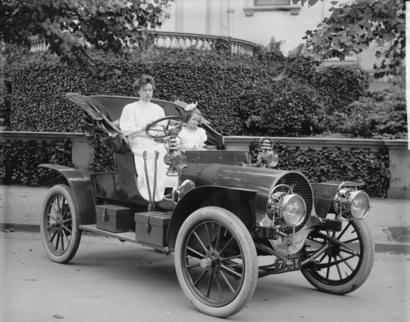
\includegraphics[width=\linewidth]{sample-franklin}
  \caption{1907 Franklin Model D roadster. Photograph by Harris \&
    Ewing, Inc. [Public domain], via Wikimedia
    Commons. (\url{https://goo.gl/VLCRBB}).}
  \Description{A woman and a girl in white dresses sit in an open car.}
\end{figure}

Your figures should contain a caption which describes the figure to
the reader. These figure captions are placed {\itshape below} the figure.

Every figure should also have a figure description unless it is purely
decorative. These descriptions convey what is in the image to someone
who cannot see it. These descriptions are used by search engine crawlers for
indexing images. Additionally, the description is shown when images cannot be loaded.

A figure description (entered using \texttt{{\textbackslash}Description}\{\}) must be \emph{unformatted} plain text less than 2000
characters long (including spaces).  {\bfseries Figure descriptions
  should not repeat the figure caption – their purpose is to capture
  important information that is not already provided in the caption or
  the main text of the paper.} For figures that convey important and
complex new information, a short text description may not be
adequate. More complex alternative descriptions can be placed in an
appendix and referenced in a short figure description. For example,
provide a data table capturing the information in a bar chart, or a
structured list representing a graph.  For additional information
regarding how best to write figure descriptions and why doing this is
so important, please see
\url{https://www.acm.org/publications/taps/describing-figures/}.

\section{Citations and Bibliographies}

The use of \BibTeX\ for the preparation and formatting of your
references is strongly recommended. Authors' names should be complete
--- use full first names (``Donald E. Knuth'') not initials
(``D. E. Knuth'') --- and the salient identifying features of a
reference should be included: title, year, volume, number, pages,
article DOI, etc.

The bibliography is included in your source document with these two
commands, placed just before the \verb|\end{document}| command:
\begin{verbatim}
  \bibliographystyle{ACM-Reference-Format}
  \bibliography{bibfile}
\end{verbatim}
where ``\verb|bibfile|'' is the name, without the ``\verb|.bib|''
suffix, of the \BibTeX\ file.

Citations and references are numbered by default.
\begin{comment}
A small number of
ACM publications have citations and references formatted in the
``author year'' style; for these exceptions, please include this
command in the {\bfseries preamble} (before the command
``\verb|\begin{document}|'') of your \LaTeX\ source:
\begin{verbatim}
  \citestyle{acmauthoryear}
\end{verbatim}
\end{comment}
Some examples are:  A paginated journal article \cite{Abril07}, an
  enumerated journal article \cite{Cohen07}, a reference to an entire
  issue\,\cite{JCohen96}, a monograph (whole book) \cite{Kosiur01}, a
  monograph/whole book in a series (see 2a in spec. document) \cite{Harel79}, a divisible-book such as an anthology or compilation
  \cite{Editor00} followed by the same example, however we only output
  the series if the volume number is given \cite{Editor00a} (so
  Editor00a's series should NOT be present since it has no vol. no.),
  a chapter in a divisible book \cite{Spector90}, a chapter in a
  divisible book in a series \cite{Douglass98}, a multi-volume work as
  book \cite{Knuth97}, a couple of articles in a proceedings (of a
  conference, symposium, workshop for example) (paginated proceedings
  article) \cite{Andler79, Hagerup1993}, a proceedings article with
  all possible elements \cite{Smith10}, an example of an enumerated
  proceedings article \cite{VanGundy07}, an informally published work
  \cite{Harel78}, a couple of preprints \cite{Bornmann2019,
    AnzarootPBM14}, a doctoral dissertation \cite{Clarkson85}, a
  Master's thesis: \cite{anisi03}, an online document / world wide web
  resource \cite{Thornburg01, Ablamowicz07, Poker06}, a video game
  (Case 1) \cite{Obama08} and (Case 2) \cite{Novak03} and \cite{Lee05}
  and (Case 3) a patent \cite{JoeScientist001}, work accepted for
  publication \cite{rous08}, 'YYYYb'-test for prolific author
  \cite{SaeediMEJ10} and \cite{SaeediJETC10}. Other cites might
  contain 'duplicate' DOI and URLs (some SIAM articles)
  \cite{Kirschmer:2010:AEI:1958016.1958018}. Boris / Barbara Beeton:
  multi-volume works as books \cite{MR781536} and \cite{MR781537}. A
  couple of citations with DOIs:
  \cite{2004:ITE:1009386.1010128,Kirschmer:2010:AEI:1958016.1958018}. Online
  citations: \cite{TUGInstmem, Thornburg01, CTANacmart}. Artifacts:
  \cite{R} and \cite{UMassCitations}.

\section{Quotations}
Quotations may be italicized when \textit{``placed inline''}. While longer quotations can be placed in a \verb|quote| environment, as shown below:

\begin{quote}
Longer quotes, when placed in their own paragraph, need not be
italicized or in quotation marks when indented.  
\end{quote}

\section{Language, Style, and Content}

Spelling and
punctuation may use any dialect of English (e.g., British, Canadian,
US, etc.) provided this is done consistently. Hyphenation is
optional. To ensure suitability for an international audience, please
pay attention to the following:

\begin{itemize}
\item Write in a straightforward style.
\item Try to avoid long or complex sentence structures.
\item Use common and basic vocabulary (e.g., use the word ``unusual'' rather than the word ``arcane''.
\item Briefly define or explain all technical terms that may be
  unfamiliar to readers.
\item Explain all acronyms the first time they are used in your
  text---e.g., ``Digital Signal Processing (DSP)''. You might want to use the package \texttt{glossaries} to help with this.
\item Explain local references (e.g., not everyone knows all city
  names in a particular country).
\item Explain ``insider'' comments. Ensure that your whole audience
  understands any reference whose meaning you do not describe (e.g.,
  do not assume that everyone has used a Macintosh or a particular
  application).
\item Explain colloquial language and puns. Understanding phrases like
  ``red herring'' may require a local knowledge of English.  Humor and
  irony are difficult to translate.
\item Use unambiguous forms for culturally localized concepts, such as
  times, dates, currencies, and numbers (e.g., ``1--5--97'' or
  ``5/1/97'' may mean 5 January or 1 May, and ``seven o'clock'' may
  mean 7:00 am or 19:00). For currencies, indicate equivalences:
  ``Participants were paid {\fontfamily{txr}\selectfont \textwon}
  25,000, or roughly US \$22.''
\item Be careful with the use of gender-specific pronouns (he, she)
  and other gendered words (chairman, manpower, man-months). Use
  inclusive language that is gender-neutral (e.g., she or he, they,
  s/he, chair, staff, staff-hours, person-years). See the
  \textit{Guidelines for Bias-Free Writing} for further advice and
  examples regarding gender and other personal
  attributes~\cite{Schwartz:1995:GBF}. Be particularly aware of
  considerations around writing about people with disabilities.  See also ACM Diversity and Inclusion Council's web page on ``Words Matter: Alternatives for Charged Terminology in the Computing Profession''~\cite{ACMdiversity}.
\item If possible, use the full (extended) alphabetic character set
  for names of persons, institutions, and places (e.g.,
  Gr{\o}nb{\ae}k, Lafreni\'ere, S\'anchez, Nguy{\~{\^{e}}}n,
  Universit{\"a}t, Wei{\ss}enbach, Z{\"u}llighoven, \r{A}rhus, etc.).
  These characters are already included in most versions and variants
  of Times, Helvetica, and Arial fonts.
\end{itemize}

\section{Accessibility}
The Executive Council of SIGCHI has committed to making SIGCHI
conferences more inclusive for researchers, practitioners, and
educators with disabilities. As a part of this goal, all authors
are asked to improve the accessibility of their
submissions, specifically, to carry out the
following five steps:
\begin{enumerate}
\item Add alternative text to all figures
\item Mark table headings
\item Add tags to the PDF
\item Verify the default language
\item Set the tab order to ``Use Document Structure''
\end{enumerate}
For more information and links to instructions and resources, please
see: \url{http://chi2016.acm.org/accessibility}.  The
\texttt{{\textbackslash}hyperref} package allows you to create well tagged PDF files,
please see the preamble of this template for an example.

\section{Producing and Testing PDF Files}

We recommend that you produce a PDF version of your document t and then test your PDF file by viewing or printing it with Adobe Acrobat Reader Version 11 or Adobe Acrobat Reader DC. This software is
widely available at no cost. Note that most
readers will use a North American/European version of Acrobat
reader, so please check your PDF accordingly.

\section{Acknowledgments}

Identification of funding sources and other support, and thanks to
individuals and groups that assisted in the research and the
preparation of the work should be included in an acknowledgment
section, which is placed just before the reference section in your
document.

This section has a special environment:
\begin{verbatim}
  \begin{acks}
  ...
  \end{acks}
\end{verbatim}
so that the information contained therein can be more easily collected
during the article metadata extraction phase, and to ensure
consistency in the spelling of the section heading.

Authors should \emph{not} prepare this section as a numbered or unnumbered {\verb|\section|}; please use the ``{\verb|acks|}'' environment.

\section{Appendices}

If your work needs an appendix, add it before the
``\verb|\end{document}|'' command at the conclusion of your source
document.

Start the appendix with the ``\verb|appendix|'' command:
\begin{verbatim}
  \appendix
\end{verbatim}
and note that in the appendix, sections are lettered, not
numbered. This document has two appendices, demonstrating the section
and subsection identification method.

%%
%% The acknowledgments section is defined using the "acks" environment
%% (and NOT an unnumbered section). This ensures the proper
%% identification of the section in the article metadata, and the
%% consistent spelling of the heading.
\begin{acks}
Thanks to all those who contributed to the \texttt{acmart} document class and earlier SIGCHI conference proceedings template.
\end{acks}

%%
%% The next two lines define the bibliography style to be used, and
%% the bibliography file.
\bibliographystyle{ACM-Reference-Format}
\bibliography{References}

%%
%% If your work has an appendix, this is the place to put it.
\appendix

\section{Research Methods}

\subsection{Part One}

Lorem ipsum dolor sit amet, consectetur adipiscing elit. Morbi
malesuada, quam in pulvinar varius, metus nunc fermentum urna, id
sollicitudin purus odio sit amet enim. Aliquam ullamcorper eu ipsum
vel mollis. Curabitur quis dictum nisl. Phasellus vel semper risus, et
lacinia dolor. Integer ultricies commodo sem nec semper.

\subsection{Part Two}

Etiam commodo feugiat nisl pulvinar pellentesque. Etiam auctor sodales
ligula, non varius nibh pulvinar semper. Suspendisse nec lectus non
ipsum convallis congue hendrerit vitae sapien. Donec at laoreet
eros. Vivamus non purus placerat, scelerisque diam eu, cursus
ante. Etiam aliquam tortor auctor efficitur mattis.

\section{Online Resources}

Nam id fermentum dui. Suspendisse sagittis tortor a nulla mollis, in
pulvinar ex pretium. Sed interdum orci quis metus euismod, et sagittis
enim maximus. Vestibulum gravida massa ut felis suscipit
congue. Quisque mattis elit a risus ultrices commodo venenatis eget
dui. Etiam sagittis eleifend elementum.

Nam interdum magna at lectus dignissim, ac dignissim lorem
rhoncus. Maecenas eu arcu ac neque placerat aliquam. Nunc pulvinar
massa et mattis lacinia.

\end{document}
\endinput
%%
%% End of file `sample-degree-report.tex'.
